\documentclass[10pt,english]{article}
\usepackage[utf8]{inputenc}
\usepackage{geometry}
\usepackage[labelfont=bf]{caption}
\usepackage{makecell}
\geometry{verbose,letterpaper,tmargin=2.54cm,bmargin=2.54cm,lmargin=2.54cm,rmargin=2.54cm}
%\geometry{verbose,letterpaper,tmargin=.1cm,bmargin=.1cm,lmargin=.1cm,rmargin=.1cm}
\usepackage{graphicx}
\DeclareGraphicsExtensions{.pdf,.png,.jpg}
\usepackage{amssymb,amsmath}
\usepackage{epstopdf}
\usepackage{tocbibind}
\usepackage[toc,page]{appendix}
\usepackage{supertabular}
\DeclareGraphicsRule{.tif}{png}{.png}{`convert #1 `dirname #1`/`basename #1 .tif`.png}
\usepackage{url}
\usepackage{subcaption}
\usepackage{caption}
\usepackage[super]{nth}
\usepackage{lineno} \linenumbers
\usepackage[doublespacing]{setspace}
\usepackage[parfill]{parskip}
\setlength{\parindent}{0pt}
\usepackage{csquotes}
\usepackage[style=apa,backend=biber,language=american]{biblatex}
\DeclareLanguageMapping{american}{american-apa}
\addbibresource{edge_sims.bib}
\DeclareFieldFormat[article]{volume}{#1}
\setlength{\bibhang}{0pt}

\usepackage{changes}
\setdeletedmarkup{\textcolor{red}{\sout{#1}}}

\begin{document}
\section*{Title page}

\textbf{Article title}: The Effect of Phylogenetic Uncertainty and Imputation on EDGE Scores

\textbf{Running Head}: Effects of Phylogenetic Uncertainty and Imputation on EDGE

\textbf{Authors:} K.\ Bodie Weedop$^{1*}$, Arne \O. Mooers$^2$, Caroline M.\ Tucker$^3$, and William D.\ Pearse$^{1}$\

$^1$ Department of Biology \& Ecology Center, Utah State University,
5305 Old Main Hill, Logan UT, 84322

$^2$ Department of Biological Sciences, Simon Fraser University, Burnaby,
British Columbia, Canada

$^3$ Department of Biology, University of North Carolina–Chapel Hill

$^*$To whom correspondence should be addressed: K.\ Bodie Weedop (\url{kbweedop@gmail.com})

\clearpage
 
\section*{Supporting Information}

\subsection*{Appendix S1: Effect of Measures of the True, Full Phylogenies}

This section contains analyses of a number of metrics from the original
phylogenies and their effect on the correlation coefficient of ED values
described in body of the manuscript.

\begin{figure}[!ht]
  \center
  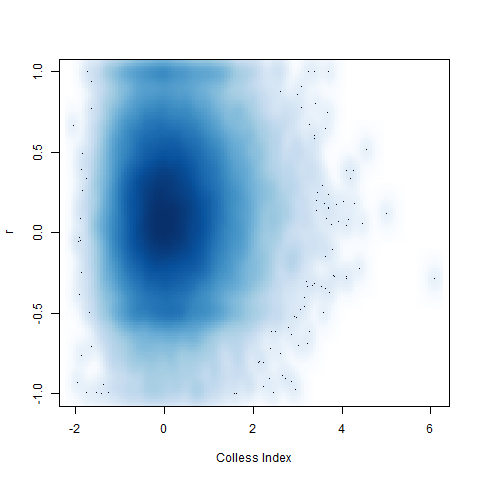
\includegraphics[width=.5\textwidth]{../figures/trueColless.png}
  \caption*{\textbf{Figure S1.1: Effect of the True Colless Index of Full Phylogeny.} 
  Smoothed color density plot of the effect of colless' index (prior to
  imputation) on the correlation coefficient of ED values. Colless' index is a
  measure of how imbalanced a tree is using the summed differences of the number
  of clades in each pair of taxa.}
\end{figure}

\begin{figure}[!ht]
  \center
  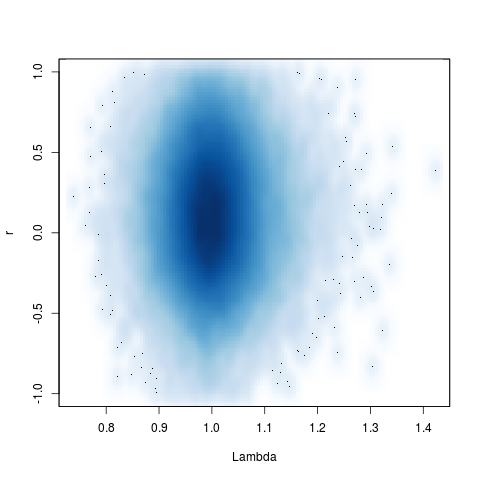
\includegraphics[width=.5\textwidth]{../figures/trueLambda.png}
  \caption*{\textbf{Figure S1.2: Effect of the True Lambda of Full Phylogeny.} 
  Smoothed color density plot of estimated speciation rate ($\lambda$; prior to
  imputation) and its effect on the correlation coefficient of ED values. }
\end{figure}

\begin{figure}[!ht]
  \center
  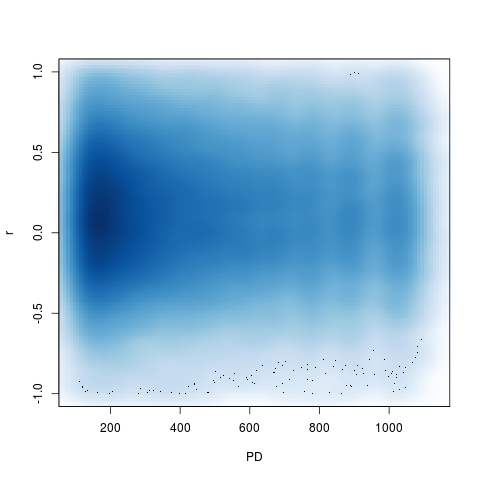
\includegraphics[width=.5\textwidth]{../figures/PD.png}
  \caption*{\textbf{Figure S1.3: Effect of True PD of Full Phylogeny.}
  Smoothed color density plot of the total phylogenetic diversity (prior to
  imputation) and its effect the correlation coefficient of ED values.}
\end{figure}

\begin{figure}[!ht]
  \center
  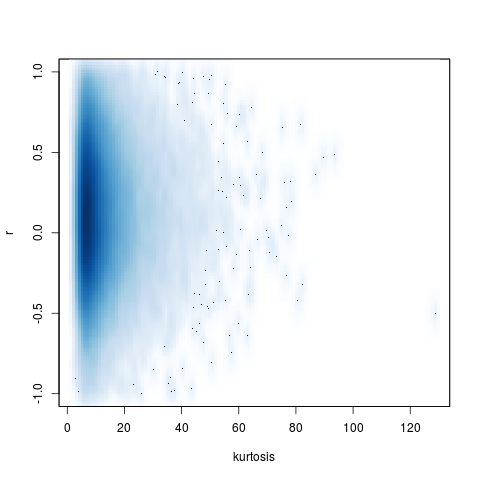
\includegraphics[width=.5\textwidth]{../figures/originalKurtosis.png}
  \caption*{\textbf{Figure S1.4: Effect of the True Kurtosis of Full Phylogeny.}
  Smoothed color density plot of kurtosis of ED values (prior to
  imputation) and its effect the correlation coefficient of ED values.}
\end{figure}

\begin{figure}[!ht]
  \center
  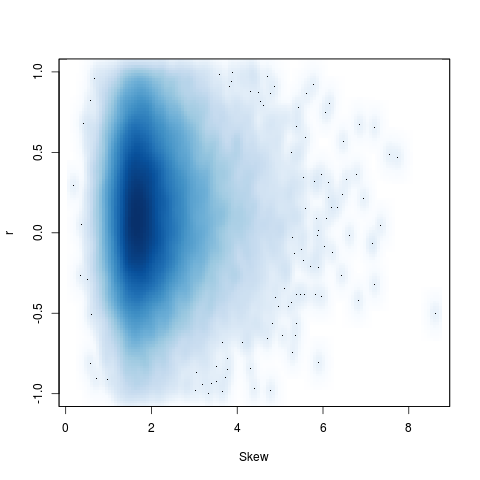
\includegraphics[width=.5\textwidth]{../figures/originalSkew.png}
  \caption*{\textbf{Figure S1.5: Effect of the True Skew of Full Phylogeny.}
  Smoothed color density plot of the skew of ED values (prior to
  imputation) and its effect the correlation coefficient of ED values.}
\end{figure}

\begin{figure}[!ht]
  \center
  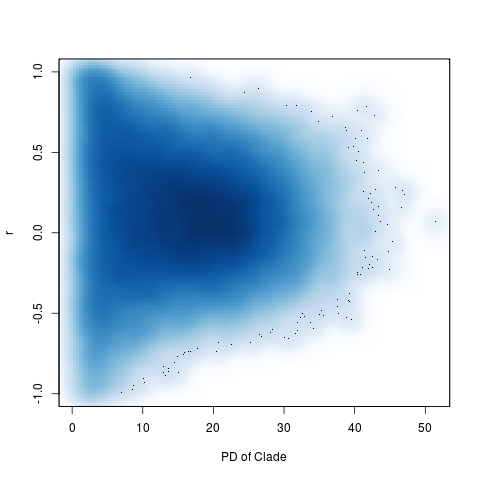
\includegraphics[width=.5\textwidth]{../figures/cladePD.png}
  \caption*{\textbf{Figure S1.6: Effect of the True PD of The Selected Clade.}
  Smoothed color density plot of the total phylogenetic diversity of the focal
  clade (prior to imputation) and its effect the correlation coefficient of ED
  values.}
\end{figure}

\clearpage
\subsection*{Appendix S2: Error Rate in Top Rankings}

This section contains plots of mean error rates in ED rankings of the top
species overall. 

\begin{figure}[!ht]
  \center
  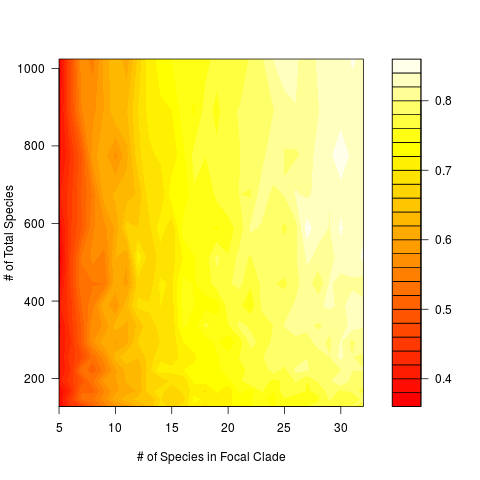
\includegraphics[width=.5\textwidth]{../figures/errorRate50.png}
  \caption*{\textbf{Figure S2.7: Mean error rate in the ranking of top 50
  species.} An interpolated heat-map of the average error rate in ED rankings of
  the top 50 species when imputing a clade of a specified size of imputed
  species. The figure shows the average error rate as a function of the total
  number of species in the phylogeny (vertical axis) and number of species in
  the focal (imputed) clade (horizontal axis). The gradient on the right gives
  the average error rate and the corresponding color.}
\end{figure}

\begin{figure}[!ht]
  \center
  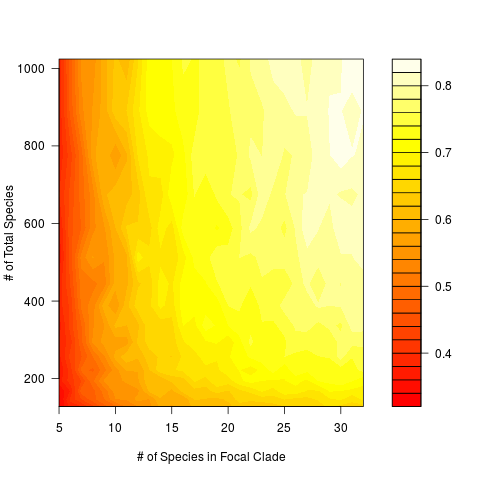
\includegraphics[width=.5\textwidth]{../figures/errorRate100.png}
  \caption*{\textbf{Figure S2.8: Mean error rate in the ranking of top 100
  species.} An interpolated heat-map of the average error rate in ED rankings of
  the top 100 species when imputing a clade of a specified size of imputed
  species. The figure shows the average error rate as a function of the total
  number of species in the phylogeny (vertical axis) and number of species in
  the focal (imputed) clade (horizontal axis). The gradient on
  the right gives the average error rate and the corresponding color.}
\end{figure}

\begin{figure}[!ht]
  \center
  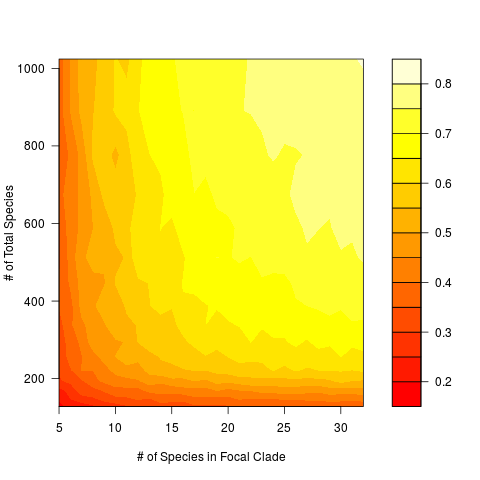
\includegraphics[width=.5\textwidth]{../figures/errorRate200.png}
  \caption*{\textbf{Figure S2.9: Mean error rate in the ranking of top 200
  species.} An interpolated heat-map of the average error rate in ED rankings of
  the top 200 species when imputing a clade of a specified size of imputed
  species. The figure shows the average error rate as a function of the total
  number of species in the phylogeny (vertical axis) and number of species in
  the focal (imputed) clade (horizontal axis). The gradient on
  the right gives the average error rate and the corresponding color.}
\end{figure}

\begin{figure}[!ht]
  \center
  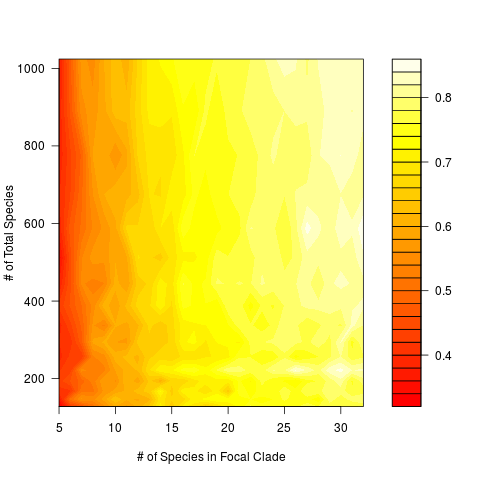
\includegraphics[width=.5\textwidth]{../figures/errorRate5pct.png}
  \caption*{\textbf{Figure S2.10: Mean error rate in the ranking of top 5\% of
  species.} An interpolated heat-map of the average error rate in ED rankings of
  the top 5\% of species when imputing a clade of a specified size of imputed
  species. The figure shows the average error rate as a function of the total
  number of species in the phylogeny (vertical axis) and number of species in
  the focal (imputed) clade (horizontal axis). The gradient on the right gives
  the average error rate and the corresponding color.}
\end{figure}

\begin{figure}[!ht]
  \center
  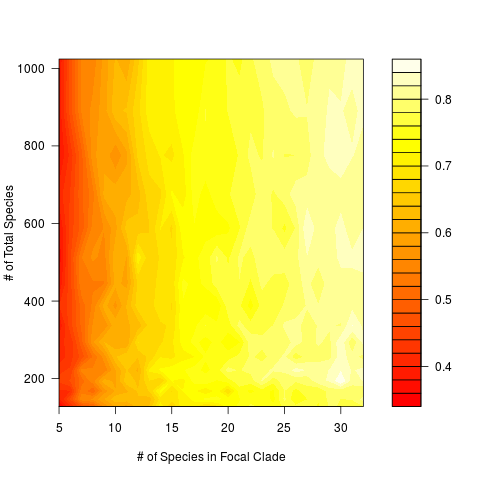
\includegraphics[width=.5\textwidth]{../figures/errorRate10pct.png}
  \caption*{\textbf{Figure S2.11: Mean error rate in the ranking of top 10\% of
  species.} An interpolated heat-map of the average error rate in ED rankings of
  the top 10\% of species when imputing a clade of a specified size of imputed
  species. The figure shows the average error rate as a function of the total
  number of species in the phylogeny (vertical axis) and number of species in
  the focal (imputed) clade (horizontal axis). The gradient on the right gives
  the average error rate and the corresponding color.}
\end{figure}

\begin{figure}[!ht]
  \center
  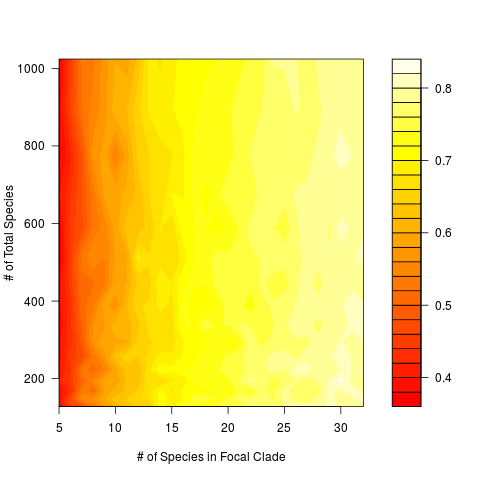
\includegraphics[width=.5\textwidth]{../figures/errorRate20pct.png}
  \caption*{\textbf{Figure S2.12: Mean error rate in the ranking of top 20\% of
  species.}An interpolated heat-map of the average error rate in ED rankings of
  the top 20\% of species when imputing a clade of a specified size of imputed
  species. The figure shows the average error rate as a function of the total
  number of species in the phylogeny (vertical axis) and number of species in
  the focal (imputed) clade (horizontal axis). The gradient on the right gives
  the average error rate and the corresponding color.}
\end{figure}
\clearpage
\subsection*{Appendix S3: Ranking Error When Using Average ED Value}

This section contains a plot of the mean ranking error when species in the focal
clades were assigned the average ED value of the clade.

\begin{figure}[!ht]
  \center
  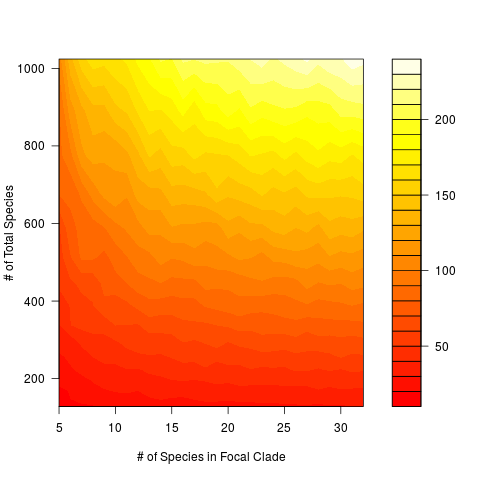
\includegraphics[width=.5\textwidth]{../figures/rankingError_avgEDforClade.png}
  \caption*{\textbf{Figure S3.13: Mean Ranking Error of Species Assigned Average
  ED.} An interpolated heat-map of the average error rate in ED rankings of the
  species in the focal clade when assigning them the average ED score for that
  clade. The figure shows the average error rate as a function of the total number
  of species in the phylogeny (vertical axis) and number of species in the focal
  (imputed) clade (horizontal axis). The gradient on the right demonstrates
  average number of positions within the full ranking that focal clade species
  shifted from their true rank.}
\end{figure}

\begin{figure}[!ht]
  \center
  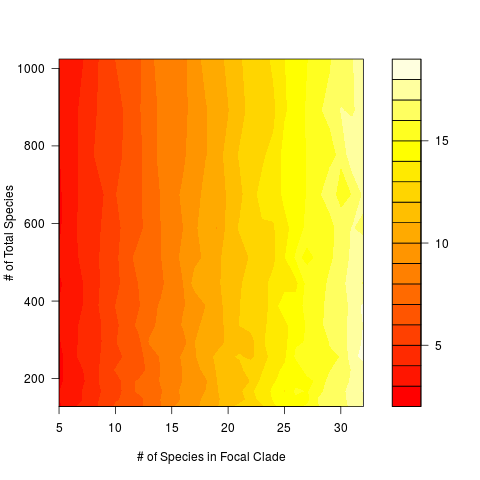
\includegraphics[width=.5\textwidth]{../figures/rankingError_remainingSpp.png}
  \caption*{\textbf{Figure S3.14: Mean Ranking Error of Non-imputed Species.}
  An interpolated heat-map of the average error rate in ED rankings of the
  species in the focal clade when assigning them the average ED score for that
  clade. The figure shows the average error rate as a function of the total
  number of species in the phylogeny (vertical axis) and number of species in
  the focal (imputed) clade (horizontal axis). The gradient on the right
  demonstrates average number of positions within the full ranking that
  non-imputed species shifted from their true rank.}
\end{figure}

\clearpage
\subsection*{Appendix S4: Figures and tables of results when using a small amount (d=0.5) of extinction}

This section contains all plots and tables that are associated with the
alternative simulations which were performed incorporating past extinction. The
underlying analyses of all plots and graphs here are identical to those that can
be seen in the main text and preceding Supporting Information appendices.  

\begin{figure}[!ht]
  \center
  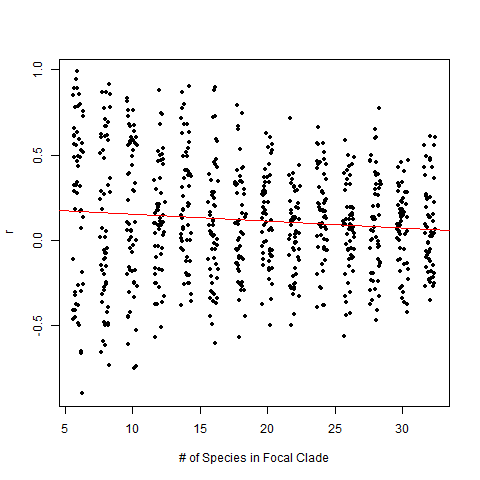
\includegraphics[width=.5\textwidth]{../figures/edModelLowExtinction.png}
  \caption{\textbf{Figure S4.15: The correlation between species' imputed and
      true ED scores plotted as a function of the number of species imputed
      (focal clade size from all sizes of phylogenies used (n = 256, ...,
      1024)).} Each data point represents the correlation between ED values
      within the focal clades where imputation has occurred, comparing species'
      true ED values with their imputed ED values. This plot, and the
      statistical analysis of it in table S4.1, show limited support for an
      association between true and imputed ED values.}
\end{figure}

\begin{table}[ht]
  \centering
  \begin{tabular}{rrrrr}
    \hline
   & Estimate & Std. Error & t value & Pr($>$$|$t$|$) \\
    \hline
    Intercept & -0.0724 & 0.5205 & -0.14 & 0.8894 \\
    Size of Focal Clade & -0.0042 & 0.0030 & -1.43 & 0.1531 \\
    Size of Phylogeny & 0.0010 & -0.01 & 0.9888 \\
    PD & 0.0001 & 0.0007 & 0.18 & 0.8544 \\
    Estimated speciation rate & 0.4050 & 0.7068 & 0.57 & 0.5669 \\
    Colless' Index & -0.0000 & 0.0000 & -0.92 & 0.3577 \\
    Skew & -0.0681 & 0.0675 & -1.01 & 0.3133 \\
    Kurtosis & 0.0083 & 0.0063 & 1.32 & 0.1878 \\
    Depth of Imputed Clade & 0.0001 & 0.0020 & 0.06 & 0.9503 \\
     \hline
\end{tabular}
\caption{\textbf{Table S4.1: Statistical model of the potential drivers of the
    correlation between imputed and true ED values when incorporating low
    (d=0.5) amounts of extinction.} Results of a multiple regression fitted to
    the data shown in figure , showing a relatively poor correlation between
    imputed and true ED scores ($F_{761,8} = 1.49$, $r^{2} = 0.005$, $p <
    0.157$). Given the extremely low predictive power, just as in the case of
    the pure birth model, of this statistical model we are reticent to make
    strong claims about drivers of the correlation between imputed and observed
    ED.}
\end{table}

\begin{figure}[!ht]
  \center
  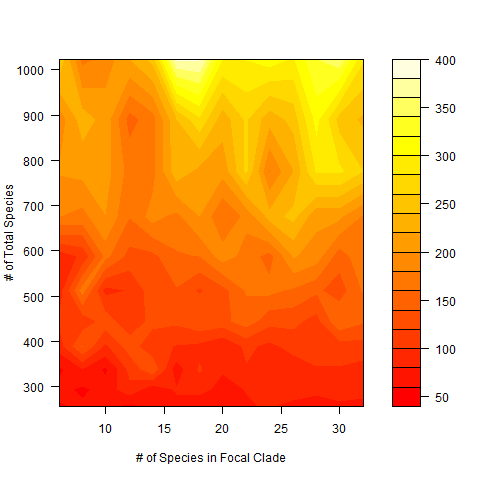
\includegraphics[width=.5\textwidth]{../figures/rankingErrorLowExtinction.png}
  \caption{\textbf{Figure S4.16: Mean ranking error of imputed species when
  incorporating low (d=0.5) amounts of extinction.} An interpolated heat-map of
  the mean ranking error of imputed species as a function of the total number of
  species in the phylogeny (vertical axis) and number of species in the focal
  (imputed) clade (horizontal axis). Table S4.2 gives statistical support for
  the trend of increased error in larger phylogenies and imputed clades.}
\end{figure}

\begin{table}[ht]
  \centering
  \begin{tabular}{rrrrr}
    \hline
   & Estimate & Std. Error & t value & Pr($>$$|$t$|$) \\ \hline
   Intercept & -1.6783 & 0.3832 & -4.38 & 0.0000 \\
   Size of focal (imputed) clade & 0.0779 & 0.0091 & 8.60 & 0.0000 \\
   Size of phylogeny & 0.5243 & 0.0144 & 36.31 & 0.0000 \\ \hline
  \end{tabular}
  \caption{\textbf{Table S4.2: Statistical model of the effect of clade and
      phylogeny size on ranking error when incorporating low (d=0.5) amounts of
      extinction.} Model of the raw data underlying figure S4.16, regressing the
      ranking error of imputed species against the number of species in the
      imputed clade and the entire phylogeny ($F_{767,2} = 696.3$, $r^2 =
      0.6439$, $p < 0.0001$). As can be seen in figure S4.16, the average
      ranking error is positively correlated with the size of the clade being
      imputed and the entire phylogeny. Square-root transformations have been
      applied to both ranking error and size of phylogeny.}
\end{table}

\clearpage
\subsection*{Appendix S5: Figures and tables of results when using a large amount (d=0.95) of extinction}

This section contains all plots and tables that are associated with the
alternative simulations which were performed incorporating past extinction. The
underlying analyses of all plots and graphs here are identical to those that can
be seen in the main text and preceding Supporting Information appendices.

\begin{figure}[!ht]
  \center
  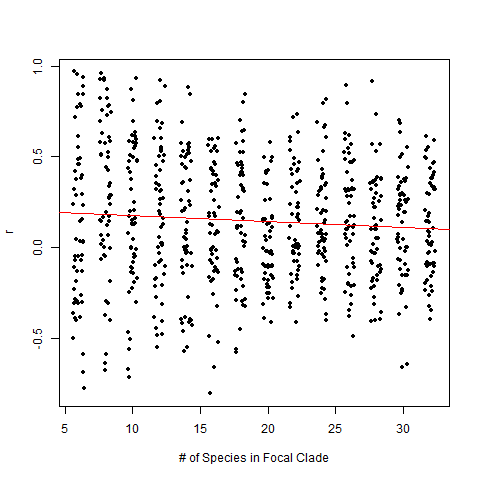
\includegraphics[width=.5\textwidth]{../figures/edModelHighExtinction.png}
  \caption{\textbf{Figure S5.17: The correlation between species' imputed and
      true ED scores plotted as a function of the number of species imputed
      (focal clade size from all sizes of phylogenies used (n = 256, ...,
      1024)).} Each data point represents the correlation between ED values
      within the focal clades where imputation has occurred, comparing species'
      true ED values with their imputed ED values. This plot, and the
      statistical analysis of it in table S5.3, show limited support for an
      association between true and imputed ED values.}
\end{figure}

\begin{table}[ht]
  \centering
  \begin{tabular}{rrrrr}
    \hline
    & Estimate & Std. Error & t value & Pr($>$$|$t$|$) \\
    \hline
    Intercept & 0.5230 & 0.1825 & 2.87 & 0.0043 \\
    Size of Focal Clade & -0.0065 & 0.0023 & -2.77 & 0.0057 \\
    Size of Phylogeny & 0.0002 & 0.0003 & 0.71 & 0.4786 \\
    PD & -0.0001 & 0.0001 & -1.17 & 0.2429 \\
    Estimated speciation rate & -0.7027 & 0.4634 & -1.52 & 0.1298 \\
    Colless' Index & 0.0000 & 0.0000 & 0.56 & 0.5746 \\
    Skew & -0.0200 & 0.0254 & -0.79 & 0.4307 \\
    Kurtosis & 0.0014 & 0.0015 & 0.99 & 0.3237 \\
    Depth of Imputed Clade & 0.0014 & 0.0008 & 1.85 & 0.0649 \\
    \hline
\end{tabular}
\caption{\textbf{Table S5.3: Statistical model of the potential drivers of the
    correlation between imputed and true ED values when incorporating high
    (d=0.95) amounts of extinction.} Results of a multiple regression fitted to
    the data shown in figure S5.17, showing a relatively poor correlation
    between imputed and true ED scores ($F_{761,8} = 1.53$, $r^{2} = 0.006$, $p
    < 0.142$). Given the extremely low predictive power, just as in the case of
    the pure birth model, of this statistical model we are reticent to make
    strong claims about drivers of the correlation between imputed and observed
    ED.}
\end{table}

\begin{figure}[!ht]
  \center
  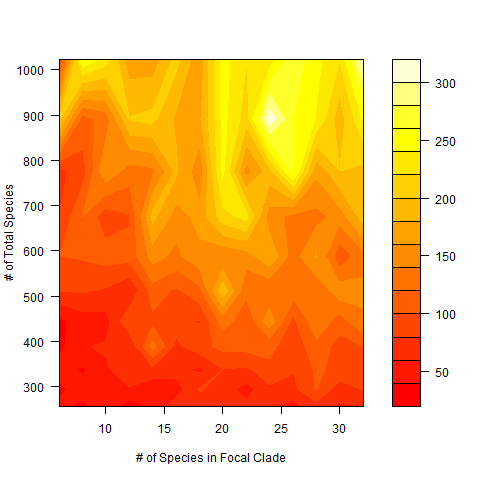
\includegraphics[width=.5\textwidth]{../figures/rankingErrorHighExtinction.png}
  \caption{\textbf{Figure S5.18: Mean ranking error of imputed species when
  incorporating high (d=0.95) amounts of extinction.} An interpolated heat-map of
  the mean ranking error of imputed species as a function of the total number of
  species in the phylogeny (vertical axis) and number of species in the focal
  (imputed) clade (horizontal axis). Table S5.4 gives statistical support for
  the trend of increased error in larger phylogenies and imputed clades.}
\end{figure}

\begin{table}[ht]
  \centering
  \begin{tabular}{rrrrr}
    \hline
    & Estimate & Std. Error & t value & Pr($>$$|$t$|$) \\ \hline
    Intercept & -2.5074 & 0.4739 & -5.29 & 0.0000 \\
    Size of focal (imputed) clade & 0.1408 & 0.0112 & 12.58 & 0.0000 \\
    Size of phylogeny & 0.4498 & 0.0179 & 25.19 & 0.0000 \\
    \hline
  \end{tabular}
  \caption{\textbf{Table S5.4: Statistical model of the effect of clade and
      phylogeny size on ranking error when incorporating low (d=0.95) amounts of
      extinction.} Model of the raw data underlying figure S5.18, regressing the
      ranking error of imputed species against the number of species in the
      imputed clade and the entire phylogeny ($F_{767,2} = 396.4$, $r^2 =
      0.507$, $p < 0.0001$). As can be seen in figure S5.18, the average
      ranking error is positively correlated with the size of the clade being
      imputed and the entire phylogeny. Square-root transformations have been
      applied to both ranking error and size of phylogeny.}
\end{table}

\end{document}